% This file was created with tikzplotlib v0.10.1.
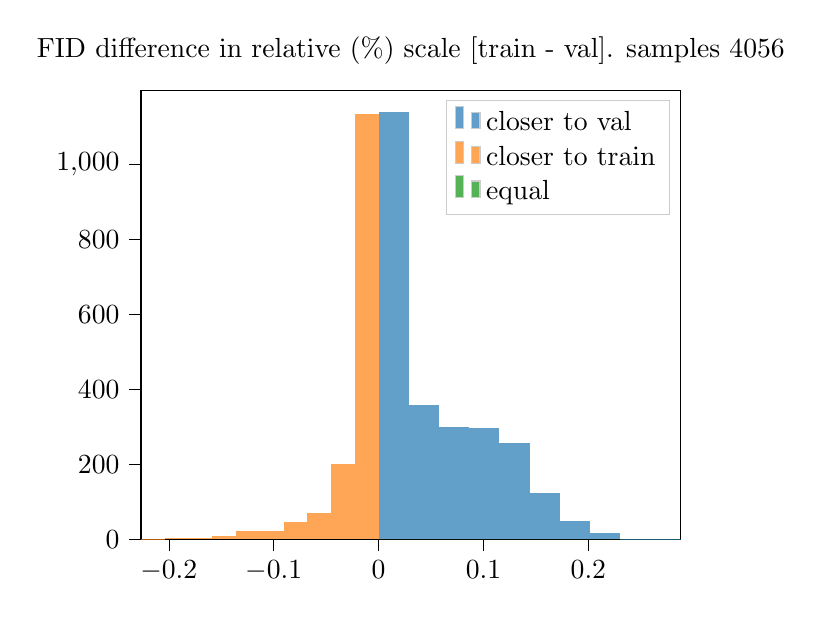
\begin{tikzpicture}

\definecolor{darkgray176}{RGB}{176,176,176}
\definecolor{darkorange25512714}{RGB}{255,127,14}
\definecolor{forestgreen4416044}{RGB}{44,160,44}
\definecolor{lightgray204}{RGB}{204,204,204}
\definecolor{steelblue31119180}{RGB}{31,119,180}

\begin{axis}[
legend cell align={left},
legend style={fill opacity=0.8, draw opacity=1, text opacity=1, draw=lightgray204},
tick align=outside,
tick pos=left,
title={FID difference in relative (\%) scale [train - val]. samples 4056},
x grid style={darkgray176},
xmin=-0.226461191049568, xmax=0.288004242339928,
xtick style={color=black},
y grid style={darkgray176},
ymin=0, ymax=1194.9,
ytick style={color=black}
]
\draw[draw=none,fill=steelblue31119180,fill opacity=0.7] (axis cs:7.03140401026557e-06,0) rectangle (axis cs:0.028806752497602,1138);
\addlegendimage{ybar,ybar legend,draw=none,fill=steelblue31119180,fill opacity=0.7}
\addlegendentry{closer to val}

\draw[draw=none,fill=steelblue31119180,fill opacity=0.7] (axis cs:0.028806752497602,0) rectangle (axis cs:0.0576064735911937,358);
\draw[draw=none,fill=steelblue31119180,fill opacity=0.7] (axis cs:0.0576064735911937,0) rectangle (axis cs:0.0864061946847854,299);
\draw[draw=none,fill=steelblue31119180,fill opacity=0.7] (axis cs:0.0864061946847854,0) rectangle (axis cs:0.115205915778377,296);
\draw[draw=none,fill=steelblue31119180,fill opacity=0.7] (axis cs:0.115205915778377,0) rectangle (axis cs:0.144005636871969,257);
\draw[draw=none,fill=steelblue31119180,fill opacity=0.7] (axis cs:0.144005636871969,0) rectangle (axis cs:0.172805357965561,122);
\draw[draw=none,fill=steelblue31119180,fill opacity=0.7] (axis cs:0.172805357965561,0) rectangle (axis cs:0.201605079059152,50);
\draw[draw=none,fill=steelblue31119180,fill opacity=0.7] (axis cs:0.201605079059152,0) rectangle (axis cs:0.230404800152744,18);
\draw[draw=none,fill=steelblue31119180,fill opacity=0.7] (axis cs:0.230404800152744,0) rectangle (axis cs:0.259204521246336,1);
\draw[draw=none,fill=steelblue31119180,fill opacity=0.7] (axis cs:0.259204521246336,0) rectangle (axis cs:0.288004242339928,1);
\draw[draw=none,fill=darkorange25512714,fill opacity=0.7] (axis cs:-0.226461191049568,0) rectangle (axis cs:-0.203816922686536,2);
\addlegendimage{ybar,ybar legend,draw=none,fill=darkorange25512714,fill opacity=0.7}
\addlegendentry{closer to train}

\draw[draw=none,fill=darkorange25512714,fill opacity=0.7] (axis cs:-0.203816922686536,0) rectangle (axis cs:-0.181172654323504,3);
\draw[draw=none,fill=darkorange25512714,fill opacity=0.7] (axis cs:-0.181172654323504,0) rectangle (axis cs:-0.158528385960472,4);
\draw[draw=none,fill=darkorange25512714,fill opacity=0.7] (axis cs:-0.158528385960472,0) rectangle (axis cs:-0.135884117597441,10);
\draw[draw=none,fill=darkorange25512714,fill opacity=0.7] (axis cs:-0.135884117597441,0) rectangle (axis cs:-0.113239849234409,22);
\draw[draw=none,fill=darkorange25512714,fill opacity=0.7] (axis cs:-0.113239849234409,0) rectangle (axis cs:-0.0905955808713766,23);
\draw[draw=none,fill=darkorange25512714,fill opacity=0.7] (axis cs:-0.0905955808713766,0) rectangle (axis cs:-0.0679513125083447,47);
\draw[draw=none,fill=darkorange25512714,fill opacity=0.7] (axis cs:-0.0679513125083447,0) rectangle (axis cs:-0.0453070441453127,71);
\draw[draw=none,fill=darkorange25512714,fill opacity=0.7] (axis cs:-0.0453070441453127,0) rectangle (axis cs:-0.0226627757822808,201);
\draw[draw=none,fill=darkorange25512714,fill opacity=0.7] (axis cs:-0.0226627757822808,0) rectangle (axis cs:-1.85074192488241e-05,1133);
\draw[draw=none,fill=forestgreen4416044] (axis cs:-6.93889390390723e-18,0) rectangle (axis cs:0.1,0);
\addlegendimage{ybar,ybar legend,draw=none,fill=forestgreen4416044}
\addlegendentry{equal}

\draw[draw=none,fill=forestgreen4416044] (axis cs:0.1,0) rectangle (axis cs:0.2,0);
\draw[draw=none,fill=forestgreen4416044] (axis cs:0.2,0) rectangle (axis cs:0.3,0);
\draw[draw=none,fill=forestgreen4416044] (axis cs:0.3,0) rectangle (axis cs:0.4,0);
\draw[draw=none,fill=forestgreen4416044] (axis cs:0.4,0) rectangle (axis cs:0.5,0);
\draw[draw=none,fill=forestgreen4416044] (axis cs:0.5,0) rectangle (axis cs:0.6,0);
\draw[draw=none,fill=forestgreen4416044] (axis cs:0.6,0) rectangle (axis cs:0.7,0);
\draw[draw=none,fill=forestgreen4416044] (axis cs:0.7,0) rectangle (axis cs:0.8,0);
\draw[draw=none,fill=forestgreen4416044] (axis cs:0.8,0) rectangle (axis cs:0.9,0);
\draw[draw=none,fill=forestgreen4416044] (axis cs:0.9,0) rectangle (axis cs:1,0);
\end{axis}

\end{tikzpicture}
